\chapter{Diseño e Implementación}

\section{Arquitectura Cliente-Servidor}

El proyecto en general está basado en la arquitectura cliente-servidor\cite{clienteservidor}. Esta arquitectura define dos roles principales que se reparten tareas de demanda y respuesta, éstos respectivamente son:

\begin{itemize}
    \item Cliente
    \item Servidor
\end{itemize}

Esta separación se produce en nuestro proyecto cuando distinguimos entre front-end (cliente) y nuestro back-end (servidor).

Nuestra interfaz haría las funciones de cliente, sería la demandante de información y nuestra API junto con la base de datos sería nuestro servidor y encargado de procesar las peticiones y responder de manera adecuada a la petición original.

Con esta disposición disponemos de la ventaja que al tener bien diferenciado el back-end, nuestra aplicación será adaptable a cualquier tipo de front-end.

La función de mantenimiento es mucho más fácil de llevar a cabo en este tipo de arquitecturas, pues si aparece algún problema en la parte de interfaz, se puede corregir sin que la corrección aplicada altere el funcionamiento de nuestro back-end o API.

\subsection{Arquitectura Cliente-Servidor y Modelo Vista Controlador}

Estas dos arquitecturas no son incompatibles, en este proyecto se han diferenciado basándonos en el MVC 3 bloques distintos con funciones asignadas: vista, controlador y modelo. 

Una vez desarrollados esos bloques, la arquitectura cliente servidor engloba en un solo bloque, llamado servidor a los bloques: controlador y modelo. La función que esta arquitectura entiende por servidor es la que se realizaría gracias a la unión de estos dos bloques.

\section{Diseño}

El diseño es un proceso que permite construir una representación abstracta del software de forma que se puedan conocer aspectos como la arquitectura, funcionalidades o la calidad antes de comenzar la codificación. Además, permite detectar problemas en etapas muy tempranas del proyecto, ahorrando costes y reduciendo la presencia de riesgos. En Scrum el diseño del software es continuo y se actualiza en cada sprint.

A continuación se mencionan algunos aspectos del diseño de la aplicación que resultan interesantes o relevantes para el correcto funcionamiento.

\subsection{Representación de los datos}

Los datos serán representados en nuestro bloque o módulo que actuará como vista. Para ello, como ya describimos en la fase de análisis, lo desarrollaremos usando el framework ReactJS.

Estos datos tienen que mostrarse en una interfaz que sea sencilla de usar, intuitiva y que se adapte a todo tipo de navegadores. 

Para la elección del aspecto de la misma, es necesaria la búsqueda de inspiración. Por lo que la interfaz de la aplicación Instagram\footnote{https://www.instagram.com/?hl=es} ha sido considerada el modelo a seguir. Observando esta interfaz en la figura \ref{fig::insta}, se puede comprobar que en cualquier momento, un usuario tiene la posibilidad de cambiar la vista general gracias a los 4 botones que contiene en el extremo inferior de la pantalla. Esta funcionalidad, será clave a la hora de buscar una plantilla que ayude para el inicio del desarrollo de nuestra interfaz. Pues, en nuestro diseño será fundamental que el usuario tenga la posibilidad de desplazarse por los distintos apartados de la aplicación siempre que lo necesite.

\begin{figure}[htbp]
    \centerline{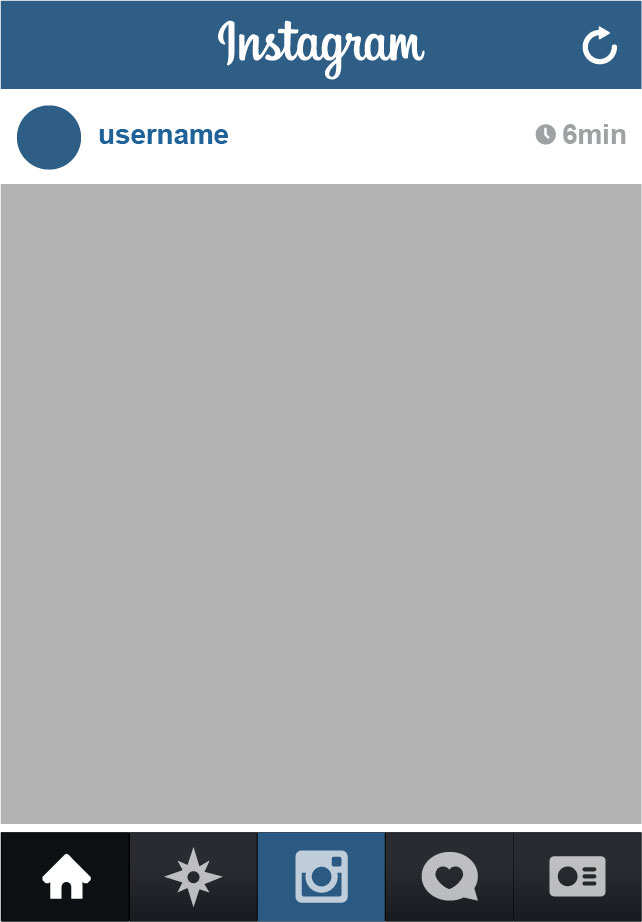
\includegraphics[width=4cm]{figuras/insta.jpg}}
    \caption{Interfaz de Instagram}
    \label{fig::insta}
\end{figure}

La idea principal es la reutilización de código con licencia de código abierto. Gracias a la comunidad de software libre, se ha encontrado una interfaz que relacione la idea descrita anteriormente junto con un diseño sencillo e intuitivo. Esta plantilla se llama \textit{adminLTE}\footnote{https://github.com/almasaeed2010/AdminLTE}, está liberada bajo la licencia de software libre \textit{MIT}\footnote{https://github.com/almasaeed2010/AdminLTE/blob/master/LICENSE} y se encuentra alojada en la plataforma GitHub.

Gracias al uso de la misma, se ha podido desarrollar una interfaz sencilla de desarrollar y agradable a la vista. En la imagen \ref{fig::rid} se puede observar como se ha desarrollado una interfaz en la que un usuario puede, en cualquier momento cambiar el contenido de la vista principal.

\begin{figure}[htbp]
    \centerline{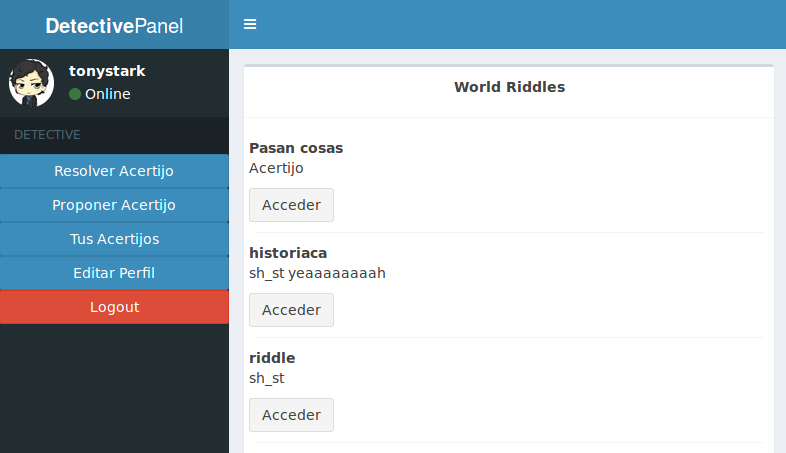
\includegraphics[width=12cm]{figuras/riddling.png}}
    \caption{Interfaz de Riddling, nuestro proyecto}
    \label{fig::rid}
\end{figure}

\subsubsection{ReactJS y sus componentes}

ReactJS es un framework que se basa en la reutilización de componentes. Un componente es cualquier estructura definida en la que se mostrará información. Cada componente se comporta como una instancia de una clase, por lo que cada uno de ellos tiene sus atributos definidos.

El procedimiento a seguir para la creación de la vista ha sido la creación y desarrollo de las 4 vistas iniciales que dispondrá nuestra aplicación:

\begin{itemize}
    \item \textbf{AcertijosView}. En este apartado se mostrarán todas las historias accesibles del sistema. Esta vista contendrá todos los componentes \textit{SmallRiddle} que posteriormente describiremos. Esta vista se puede observar en la figura \ref{fig::acertijosview}.
    \item \textbf{ProponerView}. En este apartado se mostrará un formulario para que un usuario introduzca un acertijo. Esta vista se puede observar en la figura \ref{fig::proponerview}.
    \item \textbf{TusAcertijosView}. En este apartado se mostrarán todas las historias propias de un usuario. Esta vista también contendrá todos los componentes \textit{SmallRiddle} que posteriormente describiremos. Esta vista se puede observar en la figura \ref{fig::tusacertijosview}.
    \item \textbf{EditarPerfilView}. Gracias a esta vista un usuario será capaz de administrar su perfil. Aparecerá un formulario con los datos que podrá modificar. Nótese que esta interfaz se encuentra diseñada pero actualmente se encuentra sin funcionalidad. Se puede observar en la figura \ref{fig::editarperfilview}.
\end{itemize}

\begin{figure}[hbtp] \centering
\begin{subfigure}{.6\textwidth}
    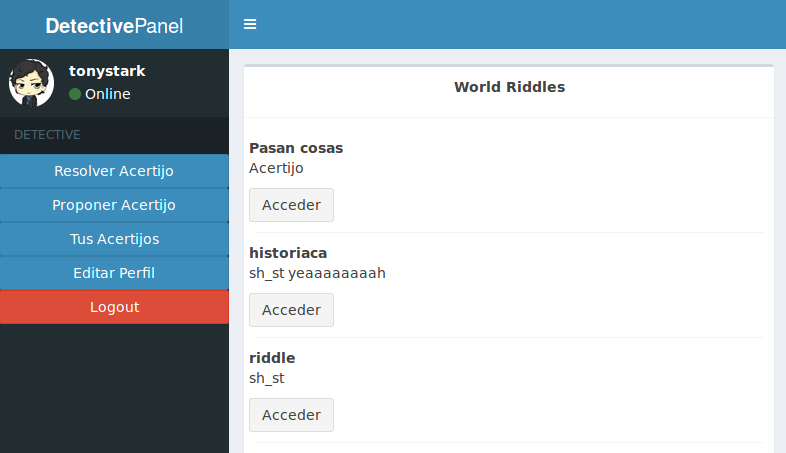
\includegraphics[width=\linewidth]{figuras/riddling.png}
    \caption{Vista AcertijosView de nuestra aplicación}
    \label{fig::acertijosview}
\end{subfigure}
\begin{subfigure}{.6\textwidth}
    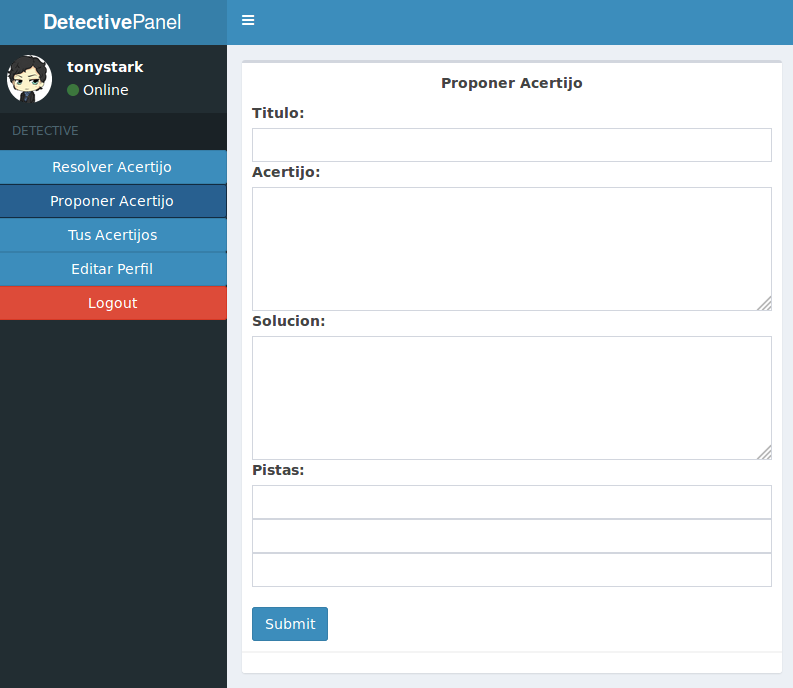
\includegraphics[width=\linewidth]{figuras/proponerview.png}
    \caption{Vista ProponerView de nuestra aplicación}
    \label{fig::proponerview}
\end{subfigure}

\begin{subfigure}{.6\textwidth}
    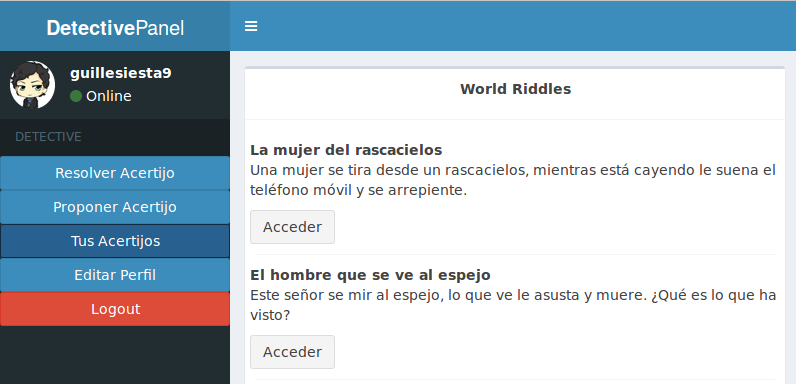
\includegraphics[width=\linewidth]{figuras/tusacertijosview.png}
    \caption{Vista de TusAcertijosView de nuestra aplicación}
    \label{fig::tusacertijosview}
\end{subfigure}

\begin{subfigure}{.6\textwidth}
    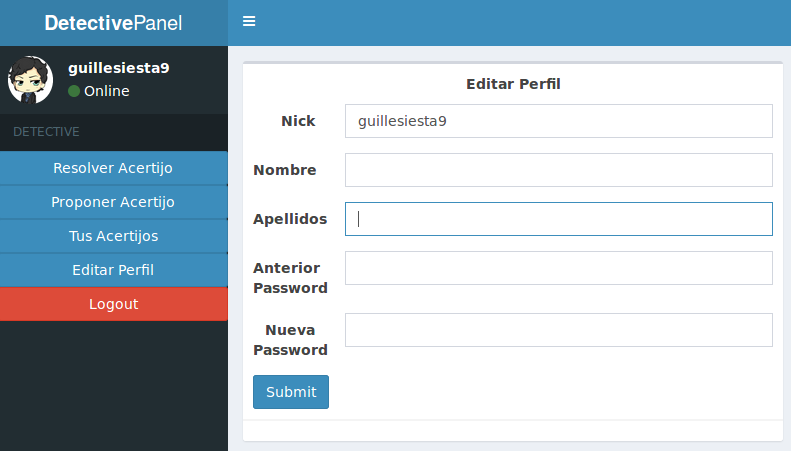
\includegraphics[width=\linewidth]{figuras/editarperfilview.png}
    \caption{Vista de EditarPerfilView de nuestra aplicación} 
    \label{fig::editarperfilview}
\end{subfigure}
\caption{Imágenes de las vistas que componen la aplicación}
\label{fig::vistas}
\end{figure}

Una vez definidas las vistas, éstas contendrán distintos tipos de componentes, que interactuarán entre ellos para poder realizar las funciones descritas en los requisitos de nuestra aplicación. Estos componentes se dividen en:

\begin{itemize}
    \item \textbf{Header}. En este componente encontramos la cabecera de la aplicación. Contiene un botón que al pulsarlo contrae hacia la izquierda el menú Sidebar. Está siempre renderizado.
    \item \textbf{Sidebar}. Este componente es el encargado de seleccionar qué vista es la que queremos escoger y visualizar. Este component se encuentra siempre accesible.
    \item \textbf{FormLogin}. El componente inicial que nos permite acceder a la plataforma.
    \item \textbf{SmallRiddle}. Es un componente que resume el título del acertijo y la descripción del mismo. Tenemos la posibilidad de acceder a él para así cargar el componente Riddle.
    \item \textbf{Riddle}. Muestra todos los datos del acertijo, a excepción de la solución. Este componente nos permite observar el estado en el que se encuentra el acertijo, la descripción del mismo, y las 3 valiosas pistas que nos ayudarán a resolverlo.
    
    Como funcionalidad adicional, este componente puede cargar todas las soluciones de ese acertijo propuestas por los usuarios y el porcentaje de cercanía con respecto a la solución final.
    \item \textbf{Solucion}. Componente que muestra el texto de la propuesta como solución de un acertijo y la puntuación otorgada por el creador del acertijo.
    \item \textbf{SolucionConCheck}. Este componente muestra la solución de un acertijo en concreto, y tiene la posibilidad de poder establecer una puntuación con respecto al porcentaje de cercanñia a la solución del acertijo. Este componente se renderiza úncamente en la vista TusAcertijosView.
\end{itemize}

En los bloques de figuras \ref{fig::componentes} y \ref{fig::componentes2} se puede observar el aspecto de cada uno de los componentes descritos.

\begin{figure}[hbtp] \centering
\begin{subfigure}{.6\textwidth}
     \centerline{
\includegraphics[width=8cm]{figuras/header.png}}
    \caption{Componente Header de nuestra aplicación}
    \label{fig::header}
\end{subfigure}
\begin{subfigure}{.6\textwidth}
    \centerline{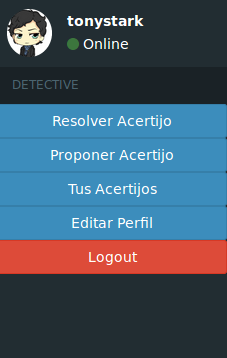
\includegraphics[width=5cm]{figuras/sidebar.png}}
    \caption{Componente Sidebar de nuestra aplicación}
    \label{fig::sidebar}
\end{subfigure}

\begin{subfigure}{.6\textwidth}
     \centerline{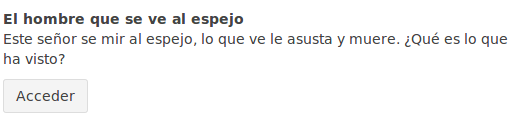
\includegraphics[width=9cm]{figuras/smallriddle.png}}
    \caption{Componente SmallRiddle de nuestra aplicación}
    \label{fig::smallriddle}
\end{subfigure}
\caption{Imágenes de los componentes que componen la aplicación}
\label{fig::componentes}
\end{figure}


\begin{figure}[hbtp] \centering
\begin{subfigure}{.6\textwidth}
     \centerline{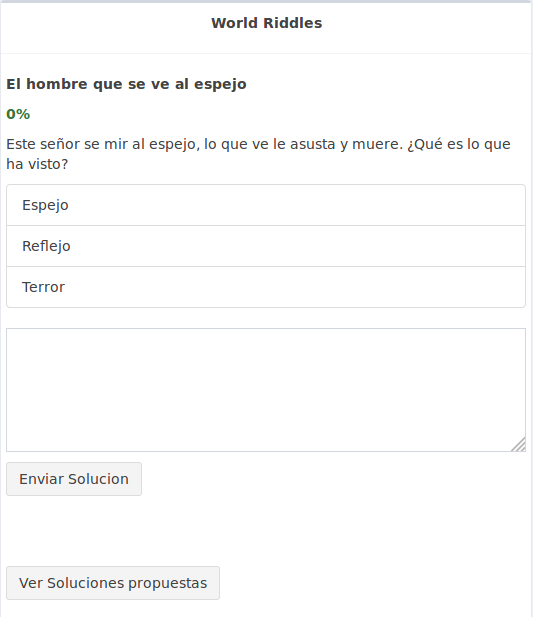
\includegraphics[width=9cm]{figuras/riddle.png}}
    \caption{Componente Riddle de nuestra aplicación} 
    \label{fig::riddle}
\end{subfigure}
\begin{subfigure}{.6\textwidth}
     \centerline{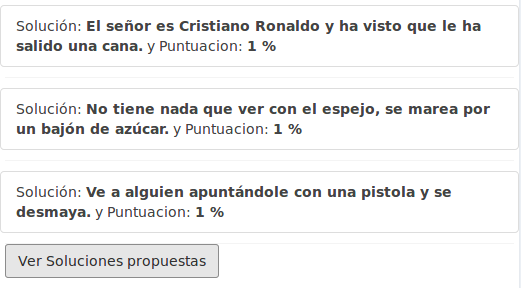
\includegraphics[width=9cm]{figuras/solucion.png}}
    \caption{Componente Solución de nuestra aplicación} 
    \label{fig::solucion}
\end{subfigure}

\begin{subfigure}{.6\textwidth}
     \centerline{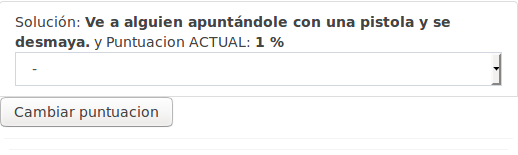
\includegraphics[width=9cm]{figuras/solucionconcheck.png}}
    \caption{Componente SoluciónConCheck de nuestra aplicación} 
    \label{fig::solucionconcheck}
\end{subfigure}
\caption{Imágenes de los componentes que componen la aplicación}
\label{fig::componentes2}
\end{figure}


\subsection{Modulado de los datos}

En esta aplicación se van a 2 distinguir dos tipos de entidades:

\begin{itemize}
    \item  Usuarios.
    \item  Acertijos.
\end{itemize}

Esto, traducido a nuestra base de datos basada en grafos, lo que estamos definiendo son 2 tipos de nodos específicos.

\begin{itemize}
    \item  \textbf{Usuarios}.
    \item  \textbf{Storie}.
\end{itemize}

Se representan en la base de datos de la la forma que muestra el bloque de imágenes \ref{fig::nodos}

\begin{figure}[hbtp] \centering
\begin{subfigure}{.6\textwidth}
     \centerline{
\includegraphics[width=2cm]{figuras/usuario.png}}
    \caption{Nodo Usuario} 
    \label{fig::riddle}
\end{subfigure}
\begin{subfigure}{.6\textwidth}
     \centerline{
\includegraphics[width=2cm]{figuras/storie.png}}
    \caption{Nodo Storie} 
    \label{fig::solucion}
\end{subfigure}
\caption{Nodos de nuestra base de datos }
\label{fig::nodos}
\end{figure}

\subsubsection{Atributos del usuario}

En la base de datos se almacenarán esta serie de atributos por nodo usuario:

\begin{itemize}
    \item \textbf{Nick}.
    \item \textbf{Contraseña}.
    \item \textbf{Nombre}.
    \item \textbf{Apellidos}.
\end{itemize}


\subsubsection{Atributos del acertijo}
En nuestra base de datos se almacenarán esta serie de atributos por nodo storie:

\begin{itemize}
    \item \textbf{Título}.
    \item \textbf{Sh\_Storie}. (acertijo)
    \item \textbf{Storie}. (solución)
    \item \textbf{Pista 1}.
    \item \textbf{Pista 2}.
    \item \textbf{Pista 3}.
\end{itemize}

\subsubsection{Relaciones entre nodos}

En el sistema se distinguen 2 tipos de relaciones:

\begin{itemize}
    \item \textbf{Escribe}. Relacionará cuando un usuario escribe un acertijo.
    \item \textbf{Propone}. Relacionará cuando un usuario propone una solución a un acertijo.
\end{itemize}

Una vez se establece el tipo de relaciones existentes en el sistema y se decida crear una relación \textit{Usuario escribe historia}, la representación gráfica sería la siguiente que se muestra en la figura \ref{fig::escribe}.

\begin{figure}
     \centerline{
\includegraphics[width=5cm]{figuras/escribe.png}}
    \caption{Relación (Usuario)-[Escribe]-(Storie)} 
    \label{fig::escribe}
\end{figure}

Neo4j nos ofrece la posibilidad de poder añadir atributos a las relaciones. Esto será útil para la relación \textit{propone}, pues en esa relación será necesario registrar el texto propuesto como solución y la puntuación de esa propuesta (inicialmente será de 1).

Esta relación quedaría representada tal y como describe la figura \ref{fig::propone}.

\begin{figure}
     \centerline{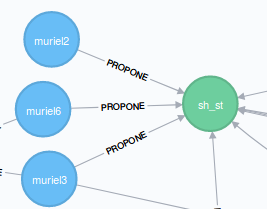
\includegraphics[width=5cm]{figuras/propone.png}}
    \caption{Relación (Usuario)-[Propone]-(Storie)} 
    \label{fig::propone}
\end{figure}

\subsubsection{Conclusión sobre el modelado de grafos y su consulta}

Como se puede observar, es realmente intuitiva y sencilla la representación gráfica que este tipo de base de dato nos propone.

Sin embargo, más sencillo  en intuitivo es aún el lenguaje \textit{Cypher} necesario para la realización de consultas. Pues éste, con una breve ojeada a su manual de usuario\footnote{https://neo4j.com/docs/developer-manual/current/cypher/}, ya se es capaz de realizar cualquier tipo de consulta necesaria para el funcionamiento de la aplicación. Por ejemplo, en el caso de que necesitáramos extraer de la base de datos todos los acertijos propuestos por el usuario "aristoteles", la consulta sería la siguiente:

\textit{MATCH (u:Usuario)-[r:Escribe]-(s:Storie) WHERE u.nick=aristoteles RETURN s.storie}

\subsection{Control de los datos}

Esta aplicación tiene que garantizar la seguridad de que todos los datos enviados y recibidos por los componentes o la base de datos son gestionados de manera adecuada. Es para ello que nuestro controlador necesitará de unos métodos a los que llamar desde nuestra interfaz.

Este controlador deberá de estar conectado a nuestra base de datos, y tendrá que ser apto al recibo de peticiones por parte de la interfaz. Nuestro controlador deberá limitarse única y exclusivamente a la ejecución de esos métodos, por lo que necesitamos que sea un sericio ligeo. Flask nos garantiza todo lo anterior.

Nuestro controlador tendrá los siguientes métodos:

\begin{itemize}
    \item \textbf{all\_stories\_titulo()}. Se devuelven todos los títulos de las historias del sistema.
    \item \textbf{user\_stories\_titulo()}. Se devuelven los títulos de las historias creadas por un usuario en concreto.
    \item \textbf{soluciones\_por\_titulo()}. Se devuelven de un acertijo todas las soluciones propuestas y su puntuación.
    \item \textbf{enviar\_comentario()}. Se añade en la base de datos la propuesta de solución de un usuario para un acertijo en concreto.
    \item \textbf{enviar\_storie()}. Se añade en la base de datos un acertijo.
    \item \textbf{cambiar\_puntuacion\_titulo()}. Se modifica en la base de datos la puntuación de una posible solución de un acertijo. Una vez cambiada la puntuación, se procederá a la actualización del estado del acertijo buscando cual es la mayor puntuación que existe de las soluciones propuestas. Esta puntuación pasará a ser el mayor de puntuación de cualquier propuesta de solución.
    \item \textbf{acertijo\_por\_titulo()}. Se busca en la base de datos el acertijo que coincida con ese título y se devuelve el texto del mismo.
    \item \textbf{storie\_por\_titulo()}. Se busca en la base de datos el acertijo que coincida con ese título y se devuelve la solución del mismo.
    \item \textbf{todo\_por\_titulo()}. Se busca en la base de datos un acertijo a partir de su título y se devuelven todos sus atributos.
    \item \textbf{login()}. Se busca en la base de datos si el usuario existe y la contraseña coincide con la registrada en el sistema.
\end{itemize}

\subsection{Flujo de los datos}

El flujo de datos puede ir desde nuestra interfaz hasta nuestra base de datos y viceversa. Para que esto ocurra, necesitamos nuestro controlador como intermediario. 

El formato de los datos estará estructurado en JSON\footnote{https://www.json.org/}, debido a su alto uso en peticiones y respuestas mediante el protocolo HTTP.

Esto es, en el caso de que desde nuestra interfaz, decidamos añadir nuestro acertijo creado, se enviará en formato JSON los datos al controlador, que extraerá la información relevante de ese JSON y añadirá lo especificado a la base de datos.

Un ejemplo de flujo de datos y pasos a seguir puede ser el ejemplo descrito en los diagramas de secuencia \ref{fig::secuencia}. En estos diagrama, se describe el funcionamiento de los eventos \textit{enviar\_storie(), enviar\_comentario(),}, en el que un usuario introduce un nuevo acertijo en el sistema.

\begin{figure}[hbtp] \centering
\begin{subfigure}{.6\textwidth}
     \centerline{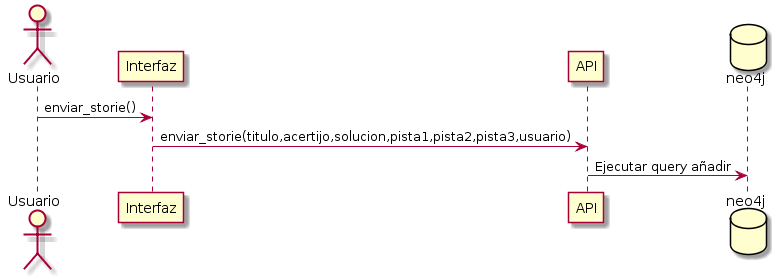
\includegraphics[width=11cm]{figuras/enviar_storie.png}}
    \caption{Diagrama de secuencia del evento enviar\_storie()} 
    \label{fig::enviarstorie}
\end{subfigure}
\begin{subfigure}{.6\textwidth}
     \centerline{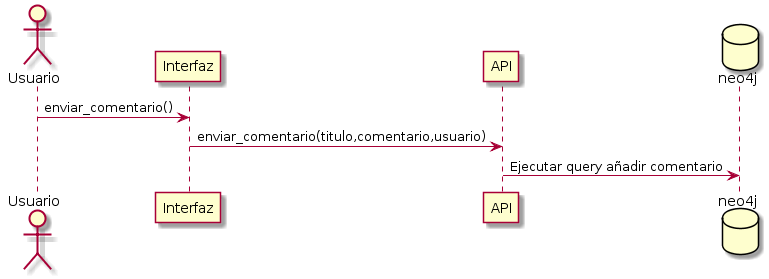
\includegraphics[width=11cm]{figuras/enviar_comentario.png}}
    \caption{Diagrama de secuencia del evento enviar\_comentario()} 
    \label{fig::enviarcomentario}
\end{subfigure}
\begin{subfigure}{.6\textwidth}
     \centerline{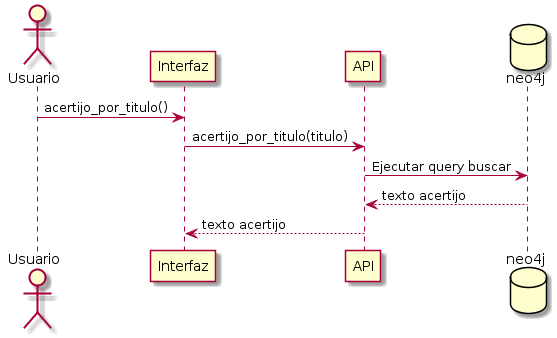
\includegraphics[width=11cm]{figuras/acertijo_por_titulo.png}}
    \caption{Diagrama de secuencia del evento acertijo\_por\_titulo()} 
    \label{fig::acertijoportitulo}
\end{subfigure}
\begin{subfigure}{.6\textwidth}
     \centerline{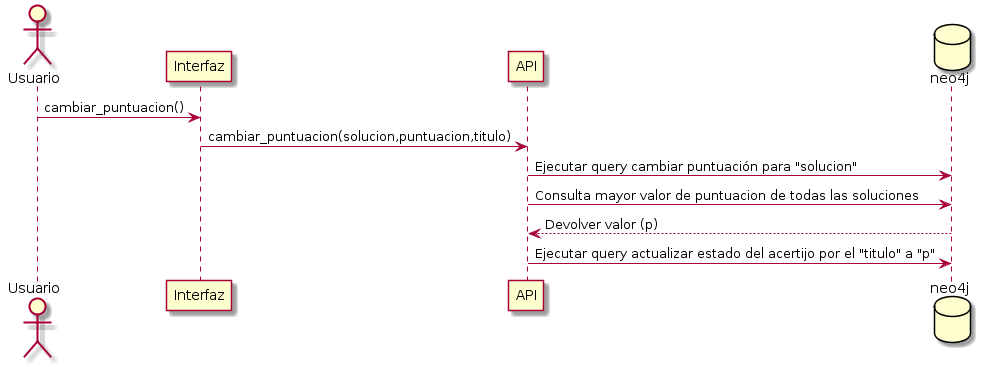
\includegraphics[width=11cm]{figuras/cambiar_puntuacion.png}}
    \caption{Diagrama de secuencia del evento cambiar\_puntuacion()} 
    \label{fig::cambiarpuntuacion}
\end{subfigure}
\caption{Diagramas de flujo de algunos eventos de la aplicación }
\label{fig::secuencia}
\end{figure}


\section{Implementación}

Una vez descrito el funcionamiento de la aplicación, el siguiente paso es la implementación. Se distinguen dos fases a la hora de llevar a cabo esta etapa. Seguiremos el orden de una primera fase en la que se desarrolla la aplicación en nuestra computadora local y otra segunda, en la que se desarrollan los automatismos necesarios para el despliegue de la aplicación creada en local.

\subsection{Implementación en local}

Para la implementación de la aplicación en local se han implementado los 3 bloques de una manera independiente. Comenzando por la instalación de nuestra base de datos, siguiendo por la creación de nuestra api y la conexión con la anterior, hasta la creación de nuestra interfaz.

\subsubsection{Base de datos}

Procedemos a instalar nuestra base de datos neo4j siguiendo el tutorial oficial. Y ya tendríamos nuestra base de datos en la dirección localhost://7474, asignada por defecto\cite{neo4jinstall}.

\subsubsection{API}

Para la creación de la API REST, se ha usado Flask, y se ha implementado este servicio de una manera cómoda y sencilla. Simplemente ejecutando el comando \textit{python nuestraapi.py} arranca el servicio local, accesible por el puerto 5000\cite{flaskinstall}.

\subsubsection{Interfaz}

Para el desarrollo de la interfaz hemos seguido el tutorial oficial para el inicio y la instalación de ReactJS. Este proceso se deberá arrancar y por defecto se situará en local en el puerto 3000.

\subsubsection{Conectando interfaz, controlador y modelo}

Una vez desarrollada cada bloque, es necesario establecer una conexión para crear el cauce por donde fluirá la información.

Para ello, en nuestra API debemos establecer primero la conexión mediante las claves ofrecidas por la base de datos\cite{connectflaskneo4j}.

Una vez conectemos, debemos instalar la librerya py2neo\footnote{https://py2neo.org/v4/} que, recomendada por la documentación oficial de neo4j, nos ayudará a la hora de hacer consultas y establecer la conexión con la base de datos.

Una vez esté el back-end conectado entre sí (API+Neo4j), procederemos a conectarlo con la interfaz.

De nuestro lado, tenemos la ventaja de que javascript (nuestro lenguaje oficial para la interfaz) dispone de una función \textit{fetch}\footnote{https://developer.mozilla.org/es/docs/Web/API/Fetch\_API/Utilizando\_Fetch}, que se encargará de realizar las peticiones HTTP a nuestra API. 

\subsection{Implementación en la nube}

A la hora de implementar en la nube, seguiremos el mismo orden que en local. 

\subsubsection{Base de datos}

Nos damos de alta en la plataforma GrapheneDB\footnote{https://www.graphenedb.com/}. Previamente exportada nuestra base de datos en local (en el caso de que queramos mantener la información) nos procedemos a la creación de una nueva base de datos en GrapheneDB. Una vez creada restauramos la nueva creación con los datos exportados de la base de datos en local\cite{graphenedb}.

Siguiendo estos sencillos pasos, ya tendríamos nuestra base de datos desplegada en la nube.


\subsubsection{API}

Para el despliegue de nuestra API en la plataforma Zeit\footnote{https://zeit.co/} necesitamos especificar que entorno será en el que nuestra API se construirá. Para ello, es necesario crear dos archivos:

\begin{itemize}
    \item \textbf{requirements.txt}\footnote{https://github.com/guillesiesta/ProjectX/blob/master/requirements.txt}. Este archivo define un entorno mediante el cual nuestra aplicación podrá ejecutar python.
    
    \item \textbf{Dockerfile}\footnote{https://github.com/guillesiesta/ProjectX/blob/master/Dockerfile}. Este archivo, nos definirá un entorno en el cual Zeit podrá crear un contenedor donde alojar nuestro servicio.
\end{itemize}

Una vez creados estos archivos, debemos comunicar en nuestra API que dejará de comunicarse por el puerto 5000 y pasará a comunicarse por el puerto 80. Para ello, habrá que añadir la siguiente línea al final del documento: \textit{app.run(host='0.0.0.0', port=80)}.

Una vez efectuados los cambios, ejecutamos desde el directorio de nuestra aplicación el comando: \textit{now} y comenzará automáticamente el despliegue. 

Zeit crea nombres de dominio aleatorios, en este caso el nombre de dominio, es decir, nuestra API o servicio estará desplegada en el dominio: \textbf{https://projectx-wvueafqhpp.now.sh/}

\subsubsection{Interfaz}

Para el despliegue en Heroku de nuestra interfaz tenemos que, primero instalar su cliente en local\cite{heroku}.

Antes, del despliegue, es necesario cambiar la dirección de todas las funciones \textit{fetch}, pues nuestra API ahora está alojada en la nube, y es la que queremos usar.

Una vez realicazos los cambios correspondientes e instalado el cliente, lo usaremos para añadir nuestro repositorio local a los repositorios de heroku\cite{heroku2}. 

Por último, procederemos al despliegue de la interfaz con el comando: \textit{heroku create}.

Automáticamente se nos desplegará una aplicación, a la que desde el panel principal de heroku se le podrá modificar el nombre, pero no la extensión que le añade heroku por defecto. Para tener un dominio propio se debería de escoger otro plan que no fuera gratuito.

La dirección oficial y, también la cconfirmación de que nuestra aplicación está alojada en la nube es: \textbf{https://riddling.herokuapp.com/}